

\chapter{Hardware --- Design e Implementação}
\label{chapter:hardware}

\begin{introduction}
Este capítulo descreve o design e a implementação do hardware nas suas quatro componentes: estrutura mecânica, sistema de atuação, sistema de controlo e microcontrolador.
\end{introduction}



\section{Estrutura Mecânica e Design 3D}
\label{sec:estrutura-mecanica}

A mesa sísmica é composta por uma base fixa, uma plataforma móvel superior e quatro colunas de suporte que ligam as duas estruturas. Estes componentes são fabricados por impressão 3D, o que permite a qualquer utilizador com acesso a uma impressora reproduzir todos os componentes.

% TODO: Ficheiro figs/prototipo_mecanico.jpg ainda não disponível — adicionar quando disponível.
\begin{figure}[h]
 \centering
 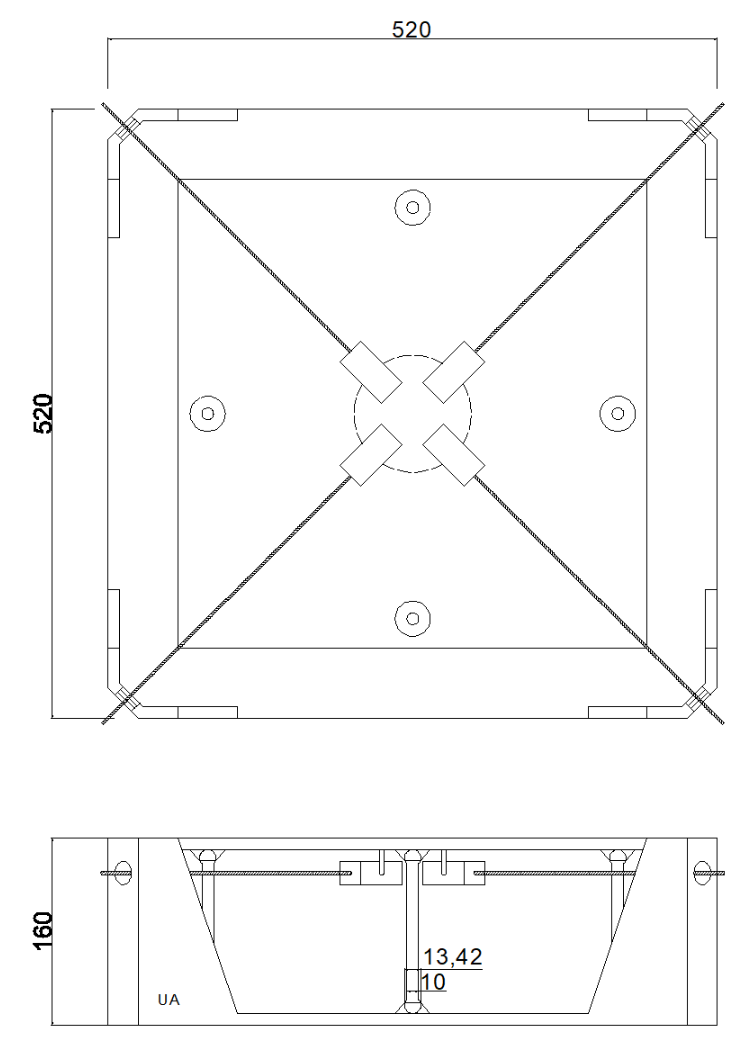
\includegraphics[scale = .3]{figs/prototipo_mecanico.png}
 \caption{Estrutura mecânica do protótipo: base fixa, plataforma móvel e quatro colunas com rótulas.}
 \label{fig:estrutura-mecanica}
\end{figure}

As rótulas instaladas em ambas as extremidades de cada coluna viabilizam o movimento bi-axial da plataforma. Ao contrário de sistemas com guias lineares rígidas separadas para cada eixo, estas rótulas permitem que a plataforma se incline livremente em qualquer direção. Quando os motores do eixo Y e os motores do eixo X empurram a plataforma em simultâneo, as colunas acomodam a combinação dos dois movimentos sem transmitir esforços parasitas à estrutura.

Cada um dos quatro motores NEMA17 está montado nas diagonais da plataforma móvel, orientado radialmente para fora. O fuso trapezoidal acoplado a cada motor encaixa numa porca trapezoidal~\cite{Fillment3DPorca} fixada na extremidade correspondente da plataforma. Quando o fuso roda, a porca avança ou recua e a plataforma desloca-se lateralmente. Os motores N e S comandam o movimento Norte-Sul e os motores E e W o movimento Este-Oeste; dentro de cada par, os dois motores rodam em sentidos opostos para que a força resultante atue no mesmo sentido sobre a plataforma.


\subsection{Escolha do Mecanismo de Translação}
\label{subsec:mecanismo-translacao}

O fuso trapezoidal~\cite{Fillment3DVarao} foi preferido à correia dentada por três razões práticas: maior força de ação disponível, menor \textit{backlash} intrínseco e melhor adequação às forças laterais que o fuso exerce sobre a plataforma. As correias dentadas, embora comuns em impressoras 3D pela sua velocidade, apresentam elasticidade que compromete a fidelidade de reprodução do perfil sísmico.

% TODO: Ficheiro figs/fuso_motor.jpg ainda não disponível — adicionar quando disponível.
\begin{figure}[h]
 \centering
 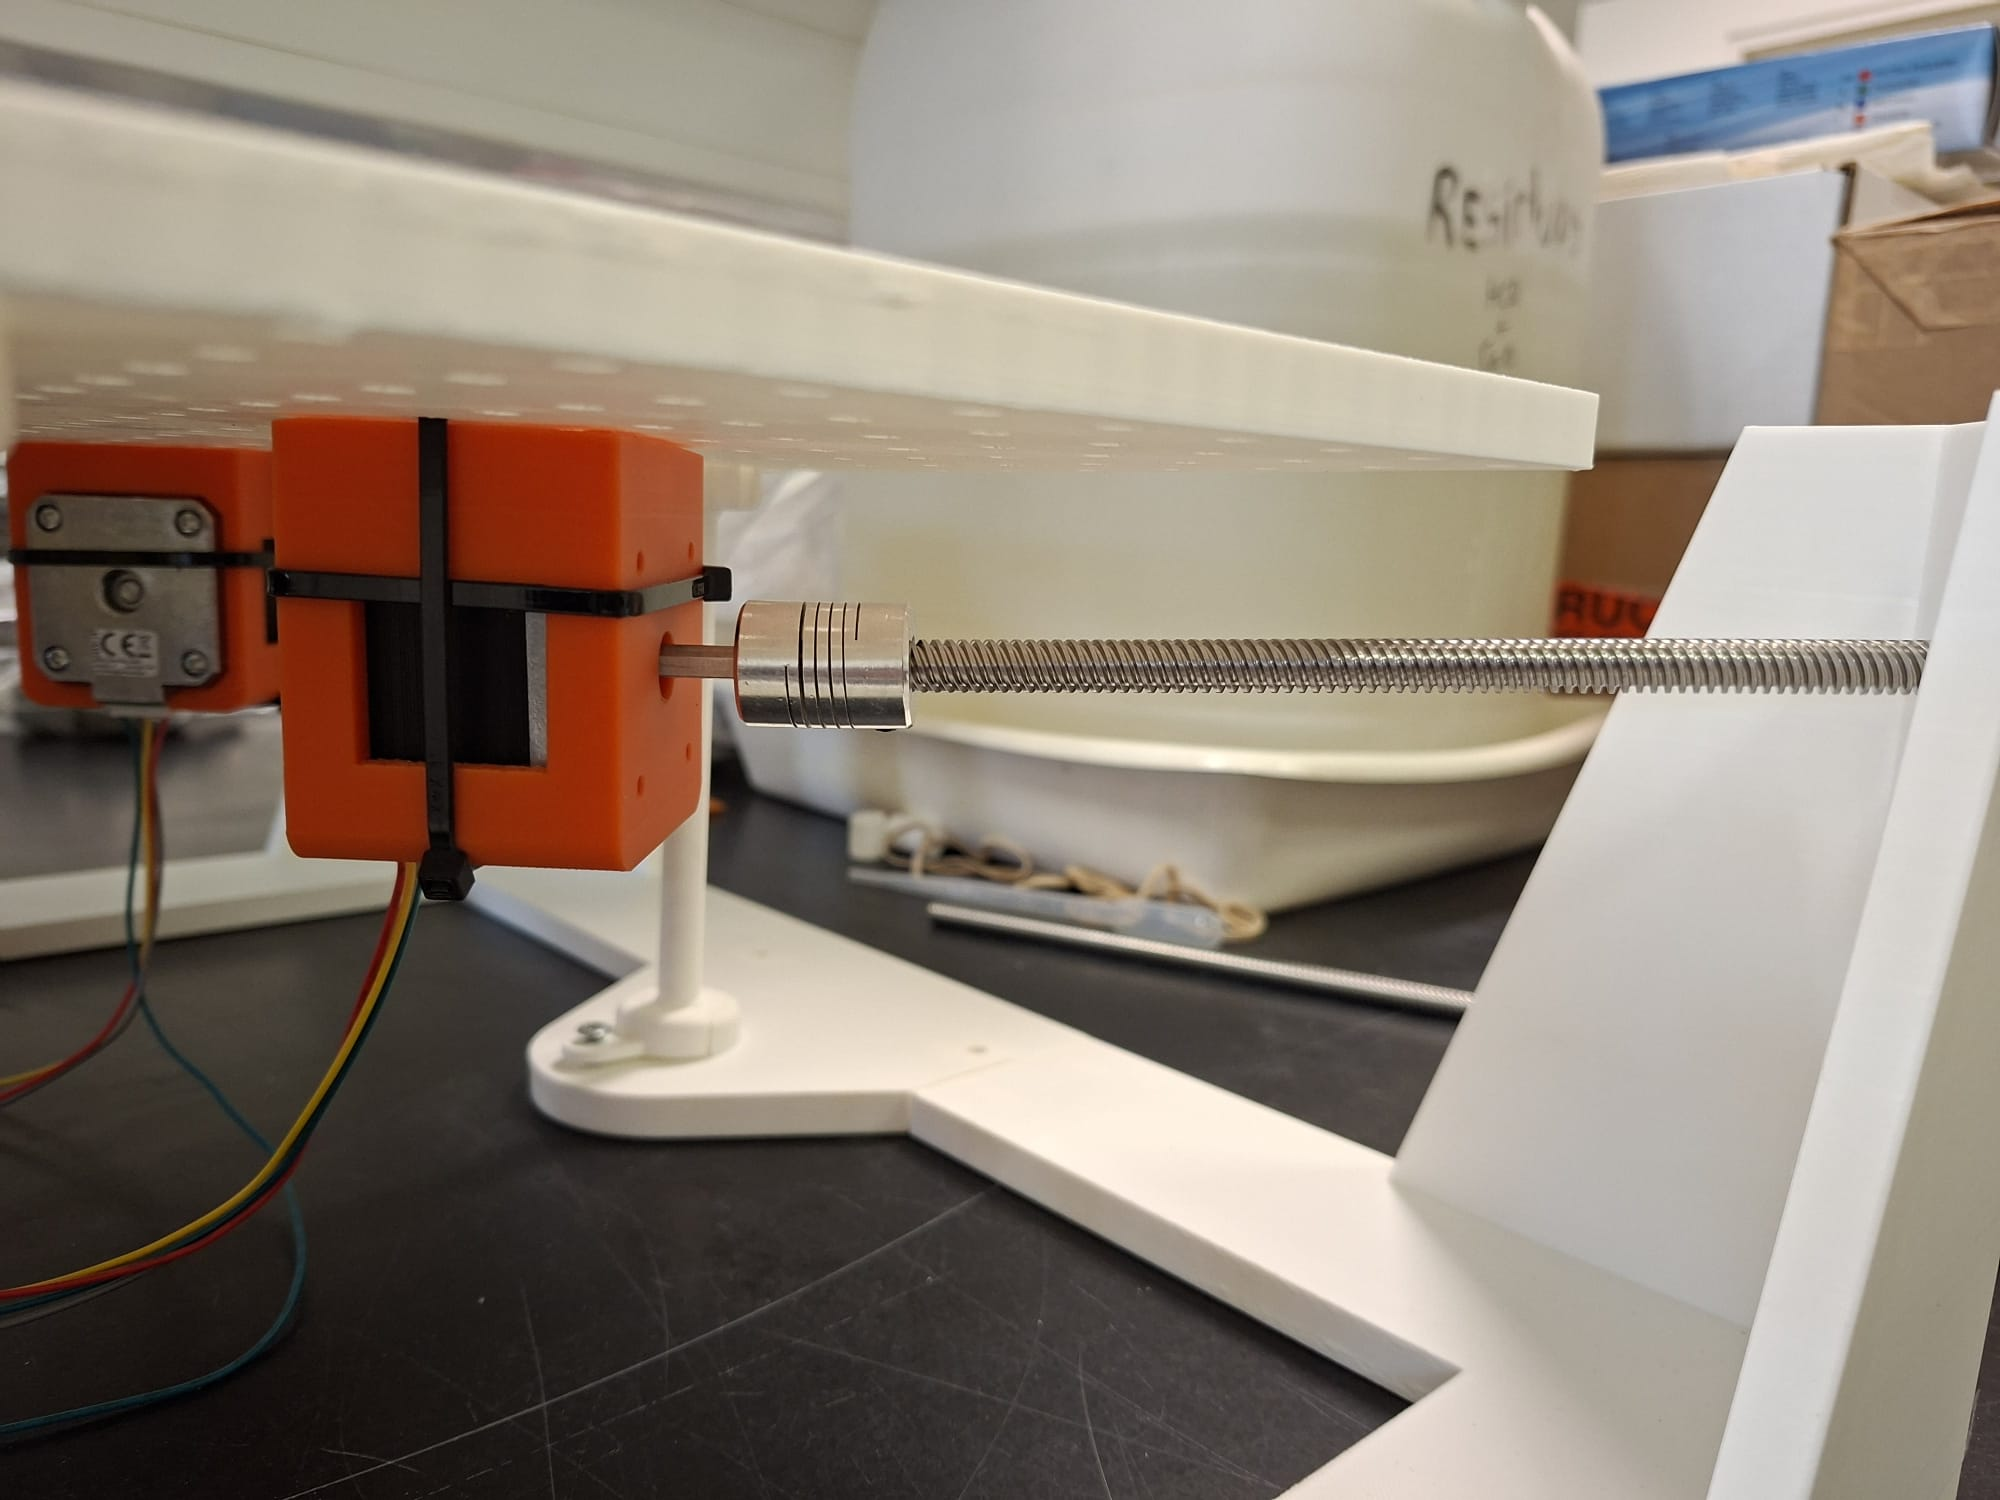
\includegraphics[width=0.5\textwidth]{figs/fuso_motor.jpeg}
 \caption{Fuso trapezoidal TR8 acoplado ao motor NEMA17.}
 \label{fig:fuso-motor}
\end{figure}

O fuso tem um \textit{lead} de 8\,mm por revolução, valor que resulta de um compromisso entre velocidade máxima atingível e resolução de posicionamento. Com um motor de 200 passos por revolução em modo \textit{full-step}, a resolução linear é de $8\,\text{mm} / 200 = 0{,}04\,\text{mm}$ por passo; com \textit{microstepping} de $1/2$, a resolução melhora para $0{,}02\,\text{mm}$ por passo.


\subsection{Modelação e Impressão 3D}
\label{subsec:modelacao-3d}

As peças estruturais são impressas em PLA. As principais são a base fixa (composta por várias partes), a plataforma superior, os suportes dos motores, os suportes das colunas e os acoplamentos motor-fuso. As colunas foram dimensionadas para acomodar a inclinação correspondente ao deslocamento máximo da plataforma nos dois eixos em simultâneo, sem que as rótulas atinjam os seus limites angulares. % TODO: COMPLETAR --- Indica o software CAD utilizado, o material (PLA), os parâmetros de impressão (temperatura, infill, velocidade) e o número exato de partes da base.

% TODO: Ficheiro figs/modelo_3d.png ainda não disponível — adicionar quando disponível.
% \begin{figure}[h]
%  \centering
%  \includegraphics[width=0.75\textwidth]{figs/modelo_3d.png}
%  \caption{Modelo 3D das peças principais da mesa sísmica.}
%  \label{fig:modelo-3d}
% \end{figure}

\section{Sistema de Atuação --- Motores NEMA17}
\label{sec:sistema-atuacao}

\subsection{Características dos Motores de Passo}
\label{subsec:caracteristicas-motores}

A Figura~\ref{fig:nema17-anexo} (Anexo~\ref{appendix:componentes}) mostra o motor NEMA17-04 utilizado.

Os motores NEMA17 são motores de passo bipolares com flange de montagem de 42,3\,mm $\times$ 42,3\,mm. O passo nominal é de 1{,}8\textdegree{} por passo, o que corresponde a 200 passos por revolução em modo \textit{full-step}.

Os motores utilizados são o modelo \textbf{Joy-IT NEMA17-04}~\cite{JoyITNEMA17}, motores de passo bipolares de dois fases com flange de 42\,mm. As suas especificações elétricas e mecânicas relevantes são as seguintes: corrente nominal de 1,68\,A por fase, resistência de 1,65\,$\Omega$ por fase, indutância de 3,6\,mH por fase e torque de retenção de 4,4\,kg.cm. A inércia do rotor é de 54\,g.cm\textsuperscript{2} e o peso do motor é de 0,28\,kg. O motor suporta uma temperatura ambiente entre $-20\,^\circ$C e $+50\,^\circ$C, com um aumento máximo de temperatura nos enrolamentos de $80\,^\circ$C com ambas as fases ativas. A folga radial máxima do veio é de 0,02\,mm e a folga axial de 0,08\,mm, ambas medidas com uma carga de 450\,g. A força radial máxima admissível é de 28\,N (a 20\,mm do flange) e a força axial máxima é de 10\,N.



\subsection{Cálculo de Torque e Velocidade}
\label{subsec:calculo-torque}

A velocidade instantânea de cada motor, em passos por segundo, é dada por:

\begin{equation}
v_{\text{steps/s}} = \frac{|\Delta\text{steps}|}{T_{\text{janela}}} = \frac{|\Delta\text{steps}|}{0{,}02\,\text{s}}
\label{eq:velocidade-motor}
\end{equation}

A velocidade linear equivalente da plataforma obtém-se por:

\begin{equation}
v_{\text{linear}} = \frac{v_{\text{steps/s}}}{\text{steps/rev}} \times \text{lead}
\label{eq:velocidade-linear}
\end{equation}

onde $\Delta\text{steps}$ é o número de passos na janela temporal de 20\,ms, $T_{\text{janela}} = 0{,}02\,\text{s}$ é a duração de cada janela e \textit{lead} $= 8\,\text{mm/rev}$.

Relativamente ao torque, considerando uma massa total da plataforma e do modelo de ensaio de aproximadamente 2\,kg, um coeficiente de atrito estimado de 0,15 (rótulas e fusos) e dois motores a partilhar a carga por eixo, o torque necessário por motor é estimado em cerca de 5,6\,kg.cm. Este valor excede ligeiramente o torque de retenção nominal do NEMA17-04 (4,4\,kg.cm), o que indica que a margem de segurança é reduzida com modelos próximos do limite máximo de carga. Na prática, o torque de arranque dos fusos trapezoidais é dominado pelo atrito estático, e o sistema demonstrou funcionamento estável. Recomenda-se, contudo, não exceder 1\,kg de massa do modelo de teste para garantir um funcionamento robusto.


\section{Sistema de Controlo --- CNC Shield e Drivers DRV8825}
\label{sec:sistema-controlo}

O ESP32 comunica com os quatro drivers DRV8825 através da CNC Shield, que centraliza os sinais STEP, DIR e EN e simplifica a cablagem. A alimentação dos motores, proveniente de uma fonte DC externa, é separada da alimentação lógica do ESP32, para evitar ruído nos sinais de controlo.


\subsection{Arquitetura da CNC Shield}
\label{subsec:arquitetura-cnc}

A CNC Shield \textbf{ARD-CNC-Kit2} da Joy-IT~\cite{JoyITCNCKit2} foi concebida para encaixar diretamente sobre um Arduino Uno. Uma vez que o ESP32 utilizado neste projeto tem um formato de PCB diferente, a ligação entre os dois é feita por fios individuais nos pinos correspondentes, sem perda de funcionalidade e sem necessidade de adaptação de hardware adicional.

A Figura~\ref{fig:cnc-shield-anexo} (Anexo~\ref{appendix:componentes}) ilustra a CNC Shield ARD-CNC-Kit2 com os quatro módulos DRV8825 instalados.

A shield disponibiliza quatro slots para módulos de driver (X, Y, Z e A), blocos de terminais para a ligação dos motores e um conector para a alimentação dos motores proveniente da fonte DC externa. O kit inclui quatro módulos DRV8825 com dissipadores de calor já instalados, prontos a encaixar nos slots da shield. A tensão de alimentação dos motores deve situar-se entre 12\,V e 35\,V. A shield dispõe ainda de seis entradas para fins de curso (\textit{endstops}), configuráveis via \textit{jumpers} para nível lógico alto ou baixo.

Os quatro motores ocupam os quatro slots disponíveis: o motor N está ligado ao slot X; o motor E ao slot Y; o motor S ao slot Z; e o motor W ao slot A. Esta correspondência foi definida por conveniência de cablagem e não reflete a orientação geográfica dos eixos.


\subsection{Microstepping e Configuração dos Drivers DRV8825}
\label{subsec:microstepping}

Os módulos de driver utilizados são os incluídos no kit Joy-IT ARD-CNC-Kit2~\cite{JoyITCNCKit2}, baseados no circuito integrado DRV8825 da Texas Instruments. Este CI suporta modos de \textit{microstepping} de $1$ (full-step), $1/2$, $1/4$, $1/8$, $1/16$ e $1/32$. A seleção do modo é feita pelos pinos M0, M1 e M2, configuráveis via \textit{jumpers} na CNC Shield.

O \textit{microstepping} divide cada passo nominal de 1{,}8\textdegree{} em sub-passos, o que melhora a resolução de posicionamento e reduz a vibração e o ruído mecânico do motor. Em modo $1/8$, cada passo nominal fica dividido em 8 sub-passos, o que se traduz em $200 \times 8 = 1600$ passos por revolução e uma resolução linear de $8\,\text{mm} / 1600 = 0{,}005\,\text{mm}$ por sub-passo.

O modo de \textit{microstepping} configurado nos \textit{jumpers} da CNC Shield é $1/2$, correspondendo a 400 passos por revolução e uma resolução linear de $8\,\text{mm} / 400 = 0{,}02\,\text{mm}$ por sub-passo. Esta escolha resulta de um compromisso entre resolução e velocidade: modos de \textit{microstepping} mais elevados (1/8, 1/16) aumentam a resolução mas reduzem o torque disponível e limitam a frequência máxima de passo admissível pelo driver, o que poderia comprometer a reprodução fiel dos picos de velocidade do registo sísmico. O modo $1/2$ oferece resolução suficiente para a amplitude de deslocamento em causa e preserva a margem de velocidade necessária para acompanhar o perfil de El~Centro.

A corrente máxima por fase é regulada pelo potenciómetro de tensão de referência (V\textsubscript{ref}) em cada módulo. Para os módulos DRV8825 genéricos com resistência de \textit{sense} de 0,1\,$\Omega$, a relação é:

\begin{equation}
I_{\text{max}} = \frac{V_{\text{ref}}}{5 \times R_{\text{sense}}} = \frac{V_{\text{ref}}}{0{,}5} = 2 \times V_{\text{ref}} \quad [\text{A}]
\label{eq:corrente-drv8825}
\end{equation}

Pela Equação~\ref{eq:corrente-drv8825}, a corrente máxima por fase resultante é de $I_{\text{max}} = 2 \times 0{,}84 = 1{,}68$\,A, com V\textsubscript{ref} de 0,84\,V medido com multímetro entre o pino central do potenciómetro e GND. Este valor corresponde exatamente à corrente nominal dos motores NEMA17-04. O funcionamento fica assim dentro das especificações do fabricante, sem risco de sobreaquecimento dos enrolamentos em regime contínuo.


\subsection{Mapeamento de Pinos ESP32 para CNC Shield}
\label{subsec:mapeamento-pinos}

O módulo ESP32 utilizado está ilustrado na Figura~\ref{fig:esp32-anexo} (Anexo~\ref{appendix:componentes}).

Os sinais STEP e DIR seguem a convenção padrão dos motores de passo: o pino DIR define o sentido de rotação (HIGH ou LOW) e cada flanco ascendente no pino STEP avança o motor um passo (ou sub-passo em modo \textit{microstepping}). A biblioteca AccelStepper gere automaticamente estes sinais com base nas instruções de velocidade recebidas pelo firmware.


\section{Microcontrolador --- ESP32}
\label{sec:microcontrolador}

% TODO: Inserir foto do módulo Joy-IT NodeMCU-ESP32-C.
\begin{figure}[h]
 \centering
 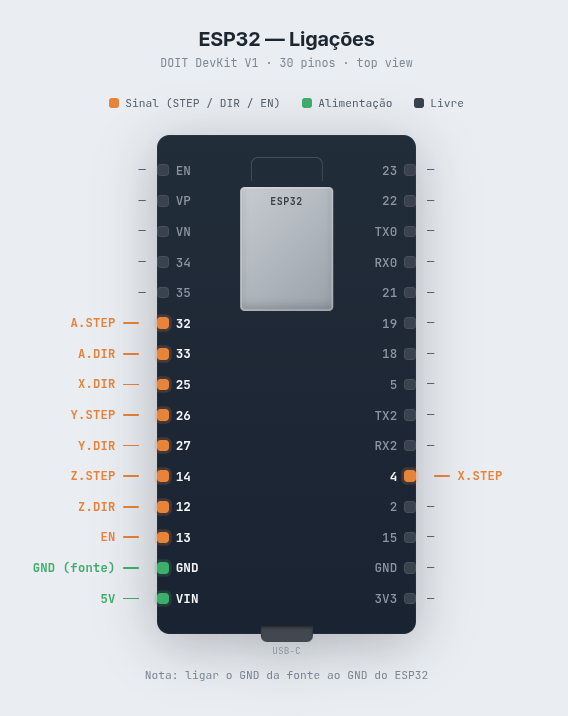
\includegraphics[width=0.4\textwidth]{figs/esp_con.png}
 \caption{Mapa de conecções entre ESP e CNC Shield.}
 \label{fig:esp32}
\end{figure}

O microcontrolador utilizado é o \textbf{Joy-IT SBC-NodeMCU-ESP32-C}~\cite{JoyITESP32}, uma placa de desenvolvimento compacta baseada no SoC ESP32 da Espressif Systems, com interface USB-C. Este módulo integra processador dual-core Xtensa LX6 a 240\,MHz, 512\,kB de SRAM, 4\,MB de memória \textit{flash}, conectividade Wi-Fi 2,4\,GHz e Bluetooth, e 21 pinos GPIO programáveis, dos quais dez são usados neste projeto para os sinais STEP, DIR e EN dos quatro motores. A programação é feita diretamente pelo Arduino IDE, o que o torna compatível com a biblioteca AccelStepper e com o ecossistema de desenvolvimento já utilizado em projetos similares de baixo custo.

A Figura~\ref{fig:esp32-anexo} (Anexo~\ref{appendix:componentes}) ilustra o ESP utilizado.



\subsection{Alimentação e Ligações}
\label{subsec:alimentacao-ligacoes}

Durante o desenvolvimento e operação normal, o ESP32 é alimentado pela porta USB (5\,V), que fornece igualmente a interface de programação via Arduino IDE e a porta série para telemetria. Esta ligação é suficiente para o funcionamento da lógica do ESP32 e dos drivers DRV8825, dado que a alimentação dos enrolamentos dos motores é assegurada por uma fonte DC externa dedicada.

Os motores são alimentados pela fonte de alimentação DC externa ORNO OR-ZL-1636~\cite{FonteMauser}, com tensão de saída de 12\,V e corrente máxima de 16,5\,A (200\,W), compatível com a gama de entrada da CNC Shield (12--35\,V)~\cite{JoyITCNCKit2}. A corrente total máxima exigida pelos quatro motores é de $4 \times 1{,}68\,\text{A} = 6{,}72\,\text{A}$, o que representa apenas 41\% da capacidade nominal da fonte. A margem de segurança é superior a 140\%, pelo que a fonte opera bem abaixo do seu limite térmico em qualquer regime de funcionamento.
